\documentclass[a4paper]{jpconf}
\usepackage{graphicx}
\usepackage{./definitions}
\usepackage{lineno,hyperref}
\usepackage{amsmath}
\usepackage{amsfonts}
\usepackage{amssymb}
\usepackage{amsthm}
\usepackage{mathrsfs}
\usepackage{color}
\usepackage{url}
\usepackage[numbers]{natbib}

\newcommand{\ee}[1]{{\color{red} EE:~#1}}
\newcommand{\rc}[1]{{\color{blue} RC:~#1}}

\bibliographystyle{iopart-num}

\begin{document}
\title{\texttt{thornado}-transport: IMEX schemes for two-moment neutrino transport respecting Fermi-Dirac statistics}

\author{Ran Chu}
\address{Department of Physics and Astronomy, University of Tennessee, Knoxville, TN 37996-1200}
\ead{rchu@vols.utk.edu}

\author{Eirik Endeve}
\address{Computational and Applied Mathematics Group, Oak Ridge National Laboratory, Oak Ridge, TN 37831 USA}
\address{Department of Physics and Astronomy, University of Tennessee, Knoxville, TN 37996-1200}
\address{Joint Institute for Computational Sciences, Oak Ridge National Laboratory, Oak Ridge, TN 37831 USA}
\ead{endevee@ornl.gov}

\author{Cory D. Hauck}
\address{Computational and Applied Mathematics Group, Oak Ridge National Laboratory, Oak Ridge, TN 37831 USA}
\address{Department of Mathematics, University of Tennessee, Knoxville, TN 37996-1320}
\ead{hauckc@ornl.gov}

\author{Anthony Mezzacappa}
\address{Department of Physics and Astronomy, University of Tennessee, Knoxville, TN 37996-1200}
\address{Joint Institute for Computational Sciences, Oak Ridge National Laboratory, Oak Ridge, TN 37831 USA}
\ead{mezz@utk.edu}

\author{Bronson Messer}
\address{Scientific Computing and Theoretical Physics Groups, Oak Ridge National Laboratory, Oak Ridge, TN 37831 USA}
\address{Department of Physics and Astronomy, University of Tennessee, Knoxville, TN 37996-1200}
\ead{bronson@ornl.gov}

\begin{abstract}
We develop implicit-explicit (IMEX) schemes for neutrino transport in a background material in the context of a two-moment model that evolves the angular moments of a neutrino phase-space distribution function.
Considering the upper and lower bounds that are introduced by Pauli's exclusion principle on the moments, an algebraic moment closure based on Fermi-Dirac statistics and a convex-invariant time integrator both are demanded.
A finite-volume/first-order discontinuous Galerkin(DG) method is used to illustrate how an algebraic moment closure based on Fermi-Dirac statistics is needed to satisfy the bounds.
Several algebraic closures are compared with these bounds in mind, and the Cernohorsky and Bludman closure, which satisfies the bounds, is chosen for our IMEX schemes.
For the convex-invariant time integrator, two IMEX schemes named PD-ARS have been proposed.
PD-ARS denotes a convex-invariant IMEX Runge-Kutta scheme that is high-order accurate in the streaming limit, and works well in the diffusion limit.
Our two PD-ARS schemes use second- and third-order, explicit, strong-stability-preserving Runge-Kutta methods as their explicit part, respectively, and therefore are second- and third-order accurate in the streaming limit, respectively.
The accuracy and convex-invariance of our PD-ARS schemes are demonstrated in the numerical tests with a third-order DG method for spatial discretization and a simple Lax-Friedrichs flux.
The method has been implemented in our high-order neutrino-radiation hydrodynamics (\texttt{thornado}) toolkit.
We show preliminary results employing tabulated neutrino opacities.
\end{abstract}

\section{Introduction}

Core-collapse supernovae (CCSNe) are the explosion happens at the end of a massive star's life.
They are a dominant source of heavy elements and play an important role in many astrophysical phenomena, such as neutron star and black hole formation.  
Furthermore, these explosions occur at energies and densities relevant to address fundamental questions in nuclear, particle, and gravitational physics. 
A solid theoretical framework for these explosion mechanism will illuminate explanations to many import questions in fundamental physics.

One essential part of the explosion mechanism is neutrino transport which drives the explosion.  
Neutrino transport is modeled by Boltzmann transport equation, which is partial differential equation and evolves the distribution function $f$.
Simulating the neutrino transport is finding a solution of Boltzmann transport equation for a given domain and period with an acceptable accuracy.

Solving Boltzmann transport multi-dimensional with high accuracy requirement can be expensive.
\ee{Balance physical fidelity and computational expediency?}
One alternation is sacrificing the accuracy: instead of solving Boltzmann transport equations, solve moment equation for an approximate solution.
\ee{What are moments?}
This kind method is moment method and we focus on two-moment method in this paper.

Applying two-moment method only is not sufficient to have an affordable solution when the simulating period is long.
To be precisely, neutrino interact with the background rapidly and its characteristic time scalar is so small comparing to the length of CCSNe explosion process. 
It makes the time step needed by an explicit time integrator dramatic small and a huge mount of calculation needed. 
\ee{Discuss fully implicit approach?}
To manipulate this challenge, implicit-explicit (IMEX) methods are taken into consideration.
By taking advantage of the fact that collision terms are local, IMEX methods are able to make the time integrator more efficient in diffusion dominate region.

However, price needs to be paid for the lunch.  
\ee{Nonlinear equations, closure, well-posedness of closure requires realizable moments}
\ee{What is moment realizability}
Two-moment method requires a realizability-preserving algebraic closure for fermion.
IMEX methods should be diffusion limit accurate \ee{why?}. 
The discussion of these prices drives this paper. 
\ee{Moment realizabilty and diffusion accurate IMEX scheme motivates this work}

This paper is recognized as following: Section~\ref{se:Two-MomentModel} discusses the mathematical model, algebraic closures, and realizability algebraic closures in the context of Fermi-Dirac statistics;
Section~\ref{se:SpacialDiscretization} we discuss moment realizability in the context of a first-order finite volume spatial discretization; Section~\ref{se:TimeIntegration} discusses how to construct a constraint-preserving, diffusion limit accurate IMEX (PD-ARS) scheme and two PD-ARS schemes are presented \ee{should we introduce the term PD-ARS here?}; Section~\ref{se:NumericalTests} gives the result of the numerical tests of the PD-ARSs; Section~\ref{se:Conclusion} is the conclusion section.
\section{Two-Moment Model}\label{se:Two-MomentModel}

\subsection{Transport Equations}
We consider neutrino transport through a static background, and include neutrino-matter interactions due to emission, absorption, and isoenergetic scattering.
After scaling to dimensionless units, the Boltzmann equation can be written as
\begin{equation}
  \pd{f}{t}+\vect{\ell}\cdot\nabla f
  =\f{1}{\tau}\,\cC(f),
  \label{eq:boltzmann}
\end{equation}
where the distribution function $f = f(\omega,\varepsilon,\vect{x},t)$ gives the number of neutrinos propagating in the direction $\omega\in\bbS^{2}$, with energy $\varepsilon\in\bbR^{+}$, at position $\vect{x}\in\bbR^{3}$ and time $t\in\bbR^{+}$.  
$\vect{\ell}(\omega)\in\bbR^{3}$ is the unit vector parallel to the neutrino three-momentum: $\vect{p}=\varepsilon\,\vect{\ell}$.
On the right-hand side, $\tau$ is a collision time scale.  
In opaque regions, where neutrinos have frequent interactions with the background, $\tau\ll1$.  
In transparent regions, where neutrinos rarely interact and stream freely, $\tau\gg1$.
The collision term, $\cC(f)$, which models emission, absorption, and isoenergetic scattering is given by
\begin{equation}
  \cC(f)=\xi\,\big(\,f_{0}-f\,\big)
  +(1-\xi)\,\big(\,\f{1}{4\pi}\int_{\bbS^{2}}f\,d\omega-f\,\big),
  \label{eq:collisionTerm}
\end{equation}
where $\xi = \sigma_{\Ab} / (\sigma_{\Ab}  + \sigma_{\Scatt} )$ is the ratio of the absorption opacity $\sigma_{\Ab}$ to the total opacity.  
The scattering opacity is $\sigma_{\Scatt}$.  
The limit $\xi = 1$, when $\sigma_{\Scatt} = 0$, corresponds to pure absorption, while $\xi = 0$, when $\sigma_{\Ab} = 0$, corresponds to pure scattering.  
The equilibrium distribution function for neutrinos is given by the Fermi-Dirac distribution:
\begin{equation}
  f_{0}(\vect{z})=\f{1}{e^{(\varepsilon-\mu(\vect{x}))/T(\vect{x})}+1}, 
  \label{eq:fermiDirac}
\end{equation}
where $\vect{z}:=\{\varepsilon,\vect{x}\}$, $T$ is the material temperature in energy units and $\mu$ is the neutrino chemical potential.
Both $T$ and $\mu$ depend on the spatial position $\vect{x}$.

\subsection{Two-Moment Model}

Approximate solutions to the Boltzmann equation, Eq.~\eqref{eq:boltzmann}, can be found by solving the two-moment model.
To this end, define the angular moments of the distribution function as follows:
\begin{equation}
  \big\{\,\cJ,\vect{\cH},\vect{\cK}\,\big\}(\vect{z},t)
  =\f{1}{4\pi}\int_{\bbS^{2}}f(\omega,\vect{z},t)\,\{\,1,\vect{\ell},\vect{\ell}\otimes\vect{\ell}\,\}\,d\omega.
  \label{eq:angularMoments}
\end{equation}  
The zeroth moment, $\cJ$, is referred to as the particle density.  
The first moment, $\bcH$, is the particle flux, and the second moment, $\bcK$, is proportional to the stress tensor.  
By integrating Eq.~\eqref{eq:boltzmann} over the momentum-space angular dimension we obtain equations for the zeroth and the first moments:
\begin{equation}
  \pd{\vect{\cM}}{t}+\nabla\cdot\vect{\cF}=\f{1}{\tau}\,\vect{\cC}(\vect{\cM}),
  \label{eq:momentEquations}
\end{equation}
with $\vect{\cM}=(\cJ,\vect{\cH})^{T}$, $\vect{\cF}=(\vect{\cH},\vect{\cK})^{T}$, and
\begin{equation}
  \vect{\cC}(\vect{\cM})=\vect{\eta}-\vect{\cD}\,\vect{\cM},
  \label{eq:collisionTermMoments}
\end{equation}
where $\vect{\eta}=(\xi\,f_{0},\vect{0})^{T}$, $\vect{\cD}=\mbox{diag}(\xi,\vect{I})$, and
$\vect{I}$ is the identity matrix.
Hence, the process of solving the Boltzmann equation, Eq.~\eqref{eq:boltzmann}, for the neutrino distribution function $f(\omega,\vect{z},t)$, is replaced by solving the two-moment equations for the neutrino number density, $\cJ(\vect{z},t)$, and flux, $\bcH(\vect{z},t)$.  

\subsection{Algebraic Closures}

The moment equation for $\bcH$ involves the higher moment $\bcK$ and the two-moment model is open.  
To close the two-moment model, we consider algebraic closures.  
For the two-moment model, algebraic closures give an approximation to $\bcK$ using the lower moments.  
Write
\begin{equation}
  \bcK = \vect{k} \cJ,
\end{equation}
where $\vect{k}$ is the Eddington tensor.  
By assuming that the distribution function is symmetric about a preferred direction $\widehat{\vect{h}}=\vect{\cH}/|\vect{\cH}|$, Levermore~\cite{levermore_1984} proposed a simple form for the Eddington tensor:
\begin{equation}
  \vect{k}=\f{1}{2}\big[\,\big(1-\chi\big)\,\vect{I}+\big(3\,\chi-1\big)\,\widehat{\vect{h}}\otimes\widehat{\vect{h}}\,\big],
  \label{eq:eddingtonTensor}
\end{equation}
where $\chi=\chi(\cJ,|\vect{\cH}|)$ is the Eddington factor.  
Thus, the two-moment model is closed by specifying the scalar $\chi$ in terms of $\cJ$ and $|\vect{\cH}|$.  

\subsection{Constraints on the Moments}

Neutrinos are fermions and obey the Pauli exclusion principle.  
Because of this, the neutrino distribution function is bounded; i.e.~$f \in [0,1]$.
As a result, the angular moments $\cJ$ and $\vect{\cH}$ and the Eddington factor $\chi$ satisfy the following bounds~\cite{levermore_1984,lareckiBanach_2011,kershaw_1976,shohatTamarkin_1943}: 
\begin{align}
\cJ \in[0,1], \quad &(1-\cJ)\cJ-|\vect{\cH}| \geq 0, \label{eq:MomentsBounds} \\
  \chi_{\mbox{\tiny min}}
  =\max\big(1-\f{2}{3\cJ},h^{2}\big)
  \leq & \chi \leq \min\big(1,\f{1}{3\cJ}-\f{\cJ}{1-\cJ}h^{2}\big)=\chi_{\mbox{\tiny max}},
  \label{eq:eddingtonFactorBounds}
\end{align}
where $h = |\bcH|/\cJ$ is the flux factor.  

The constraints in Eq.~\eqref{eq:MomentsBounds} define realizable moments $\bcM$.  
For fermions, realizable moments can only be constructed from a distribution satisfying the bounds $f \in [0,1]$.  
Moreover, the set of realizable moments is convex: let $\cR$ be the realizability set and $\bcM_{1}, \bcM_{2} \in \cR$, then $\lambda \bcM_{1} + (1-\lambda)\bcM_{2} \in \cR$ for any $\lambda \in [0,1]$~\cite{chu_etal_2018}.
As we will see later in Section~\ref{se:SpatialDiscretization}, this convexity makes it possible to design a realizability-preserving discretization for solving the two-moment model numerically.

The inequalities in Eq.~\eqref{eq:eddingtonFactorBounds} deserve further attention.  
They are important as those in Eq.~\eqref{eq:MomentsBounds}, in maintaining consistency of the two-moment model with respect to Fermi-Dirac statistics.  
When designing a numerical scheme for the two-moment model that maintains realizable $\bcM$, it is also necessary for the Eddington factor to satisfy the bounds in Eq.~\eqref{eq:eddingtonFactorBounds}.  

However, recently reported CCSN simulations using two-moment neutrino transport with algebraic closures have employed Eddington factors that can violate the bounds in Eq.~\eqref{eq:eddingtonFactorBounds}.  
As examples, we consider the Eddington factors discussed in~\cite{murchikova_etal_2017}, where the suitability of several algebraic closures for two-moment neutrino transport was evaluated.  
In Fig.~\ref{fig:EddingtonFactorsWithDifferentClosure}, we plot the Eddington factor versus the flux factor for two occupancies; $\cJ = 0.1$ (low occupancy) and $\cJ = 0.9$ (high occupancy).  
Of the algebraic closures plotted, few satisfy the bounds on the Eddington factor in Eq.~\eqref{eq:eddingtonFactorBounds}.  
Kershaw~\cite{kershaw_1976}, Wilson~\cite{wilson_1975,leblancWilson_1970}, Levermore~\cite{levermore_1984}, Minerbo~\cite{minerbo_1978}, and Janka~2~\cite{janka_1992} closures may work fine when the occupancy is low.  
When the occupancy is high, the Eddington factor due to these closures exceeds the upper bound for Fermi-Dirac statistics.  
The Eddington factor of Janka~1~\cite{janka_1991} may violate both the upper and lower bound on the Eddington factor.  
Only the closure due to Cernohorsky~\&~Bludman~\cite{cernohorskyBludman_1994} satisfies both the upper and lower bounds.  
This is not surprising as this is the only closure based on Fermi-Dirac statistics.  
Although the Levermore and Minerbo closures do not satisfy the bounds in Eq.~\eqref{eq:eddingtonFactorBounds}, they are widely used in simulations of neutrino transport in CCSNe and compact binary mergers; e.g., O'Connor \& Couch~\cite{oConnorCouch_2018}, Pan et al.~\cite{pan_etal_2018}, Glas et al.~\cite{glas_etal_2018}, Just et al.~\cite{just_etal_2018}, and Foucart et al.~\cite{foucart_etal_2015} use the Minerbo closure, while Vartanyan et al.~\cite{vartanyan_etal_2018}, Cabezon et al.~\cite{cabezon_etal_2018}, Kuroda et al.~\cite{kuroda_etal_2016}, and Fujibayashi et al.~\cite{fujibayashi_etal_2017} use the Levermore closure.  
When employing these closures in conditions of high occupancy, a numerical scheme may evolve the moments outside the realizable domain of Fermi-Dirac statistics given in Eq.~\eqref{eq:MomentsBounds}.
If this were to happen, the update step may give $\cJ>1$.
Considering the fact that the completed collision term contains blocking factors, i.e.~$(1-\cJ)\times$ something positive, $\cJ > 1$ would change blocking factors' sign and it would be difficult to predict the impact of the subsequent induced errors on the simulation outcome.
\rc{Besides, even with the simplified collision term, Eq~\ref{eq:collisionTermMoments}, $\cJ>1$ could result... the reason of crash}
If treatments are developed to map the unrealizable moments into the realizable domain, they should be developed to conserve lepton number, energy, and momentum.

\begin{figure}[h]
  \centering
  \begin{tabular}{cc}
    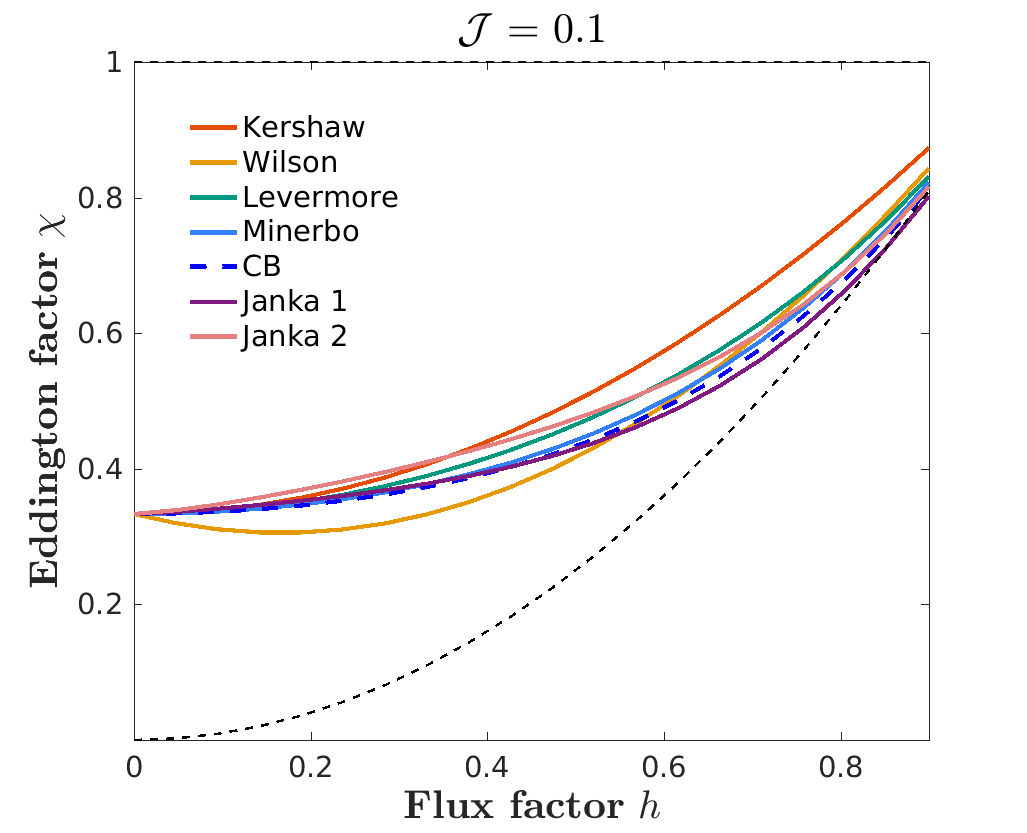
\includegraphics[width=0.5\textwidth]{figures/Closures0_10}
    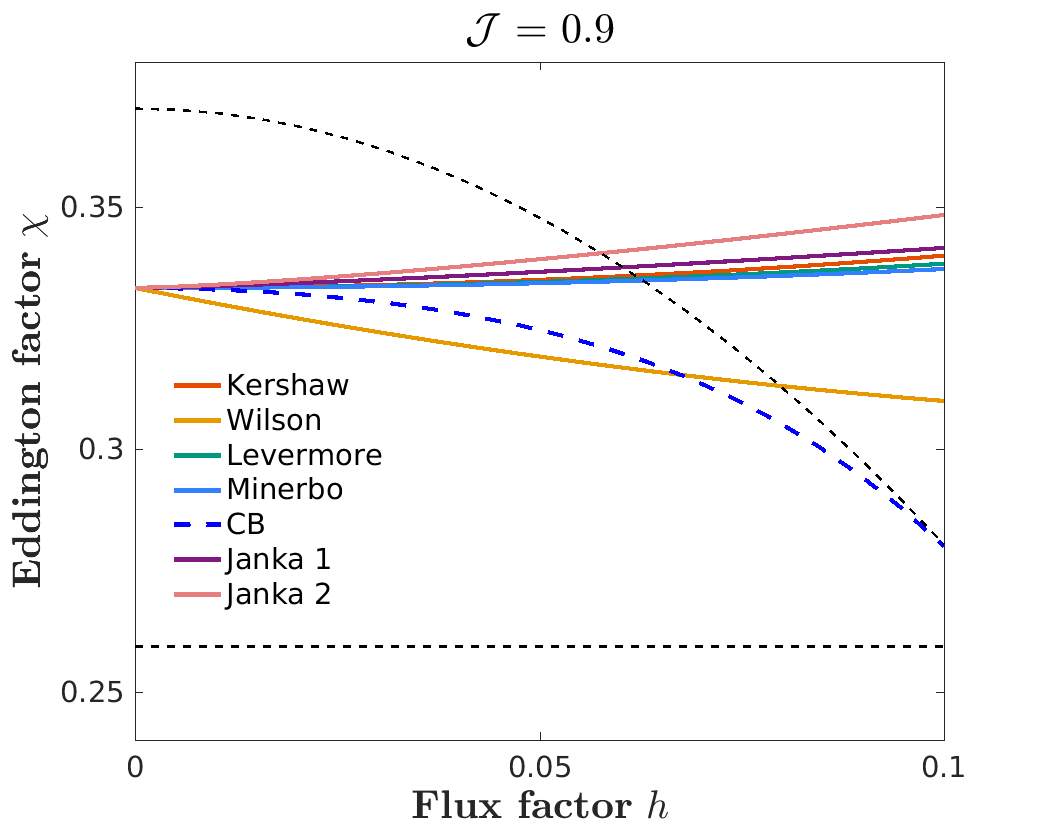
\includegraphics[width=0.5\textwidth]{figures/Closures0_90}
  \end{tabular}
   \caption{Plot of Eddington factors $\chi$ versus flux factor $h$ for different values of $\cJ$ for various algebraic closures: $\cJ=0.1$ (left panel, low occupancy) and $\cJ=0.9$ (right panel, high occupancy).  In each panel we plot the Eddington factors of two-moment closures due to Kershaw (red), Wilson (yellow), Levermore (green), Minerbo (light blue), Cernohorsky \& Bludman (blue), Janka~1 (purple), and Janka~2 (pink) .  We also plot $\chi_{\mbox{\tiny min}}$ and $\chi_{\mbox{\tiny max}}$, defined in Eq.~\eqref{eq:eddingtonFactorBounds} (lower and upper dashed black lines, respectively).}
  \label{fig:EddingtonFactorsWithDifferentClosure}
\end{figure}
\section{Spatial Discretization}\label{se:SpacialDiscretization}

In this section we discretize the two-moment model with a simple first-order finite volume method to illustrate how the closure affects the realizability-preserving property of the method.  
By assuming that the moments at time level $t^{n}$ ($\bcM^{n}$) satisfy the bounds in Eq.~\eqref{eq:MomentsBounds}, our goal is to identify sufficient conditions such that the moments at time level $t^{n+1}$ ($\bcM^{n+1}$) also satisfy the bounds.  
To simply the illustration, we limit the discussion to one spatial dimension and employ a uniform Cartesian mesh.  
(The extension to multiple spatial dimensions and high-order discretization using the discontinuous Galerkin method is given in~\cite{chu_etal_2018}.)

We divide the spatial domain $D$ into $N$ uniform cells and denote the $i$-th cell by $\bK_{i}$, with $i = 1,\ldots,N$; i.e.,
\begin{equation*}
  D = \cup_{i = 1}^{N} \bK_{i} \quad \text{with} \quad
  \bK_{i}=\{\,x : x\in(x_{i-1/2}, x_{i+1/2})\}.
\end{equation*}
Denote the cell width by $\dx = D/N$.  
The cell-average of the moments is defined as
\begin{equation}
  \bcM_{i} = \dfrac{1}{\dx} \int_{\bK_i}\bcM dx.
\end{equation}
Integrating Eq.~\eqref{eq:momentEquations} over $\bK_{i}$ gives
\begin{equation}
  \dfrac{d \bcM_{i}}{d t} = - \dfrac{1}{\dx} \left( \widehat{\bcF}(\bcM_{i},\bcM_{i+1}) -  \widehat{\bcF}(\bcM_{i-1},\bcM_{i})\right) + \f{1}{\tau}\,\cC(\bcM_{i}),
  \label{eq:SemiDiscretizatedMomentEquation}
\end{equation}
where $\widehat{\bcF}(\vect{\cM}_{a},\vect{\cM}_{b})$ is the numerical flux and $\f{1}{\tau}\,\cC(\bcM_{i})$ is the collision term evaluated with $\bcM_{i}$.
In this paper we use the global Lax-Friedrichs flux (setting the largest absolute eigenvalue of the flux Jacobian to one)
\begin{equation}
  \widehat{\bcF}_{\LF}(\vect{\cM}_{a},\vect{\cM}_{b})
  =\f{1}{2}\,\big(\,\bcF(\vect{\cM}_{a})+\bcF(\vect{\cM}_{b})-(\,\vect{\cM}_{b}-\vect{\cM}_{a}\,)\,\big).
  \label{eq:Lax-Friedrichs flux}
\end{equation}
By treating the transport term explicitly with forward Euler and the collision term implicitly with backward Euler, we have
\begin{align}
  \bcM_{i}^{n+1} = \widetilde{\bcM}^{n}_{i} + \f{\dt}{\tau}\,\cC(\bcM^{n+1}_{i}),
  \label{eq:MomentIMEX}
\end{align}
where we have defined
\begin{align}
  \widetilde{\bcM}^{n}_{i} 
  & = \bcM_{i}^{n} - \frac{\dt}{\dx} \left( \widehat{\bcF}_{\LF}(\bcM^{n}_{i},\bcM^{n}_{i+1}) -  \widehat{\bcF}_{\LF}(\bcM^{n}_{i-1},\bcM^{n}_{i})\right)\nonumber \\
  & = (1-\beta)\bcM_{i}^{n} + \beta\left[ \f{1}{2}\left( \bcM^{n}_{i+1}-\bcF(\bcM^{n}_{i+1})\right)  + \f{1}{2}\left( \bcM^{n}_{i-1}+\bcF(\bcM^{n}_{i-1})\right)\right],
  \quad\beta = \frac{\dt}{\dx}.  
\label{eq:widetildeM}
\end{align}

Consider Eq.~\eqref{eq:MomentIMEX} and assume that $\bcM_{i}^{n}$ is realizable for all $i$.  
Lemma~3 in~\cite{chu_etal_2018} states that $\bcM^{n+1}_{i}$ is realizable provided $\f{\dt}{\tau} > 0$. 
%and $\widetilde{\bcM}^{n}_{i}$ is realizable.  
In Eq.~\eqref{eq:widetildeM}, if $\beta \in [0,1]$, $\widetilde{\bcM}^{n}_{i}$ is expressed as a convex combination of $\bcM_{i}^{n}$ and the expression in the square brackets on the right-hand side of Eq.~\eqref{eq:widetildeM}.  
It follows that $\widetilde{\bcM}^{n}_{i}$ is realizable if the expression inside the square brackets is realizable.  
By Lemma~2 in~\cite{chu_etal_2018}, the expression in square brackets is realizable for a distribution satisfying $f\in[0,1]$.  
For the two-moment model considered here, realizability depends on the algebraic closure.  
Specifically, if $\bcM_{i}^{n}$ is realizable and the Eddington factor satisfies the bounds in Eq.~\eqref{eq:eddingtonFactorBounds}, then $\bcM^{n+1}_{i}$ is realizable provided $\beta \in [0,1]$.  
Thus, realizability of $\bcM^{n+1}_{i}$ requires both a closure based on Fermi-Dirac statistics and a CFL condition $\dt\le\dx$.  
\section{Time Integration} \label{se:TimeIntegration}

In this section we show how to use the property we introduced at the end of the previous section to construct a constraint-preserving implicit-explicit (IMEX) scheme.
The semi-discretization of the moment equation, Eq.~\eqref{eq:momentEquations}, results in a system of ordinary differential equations of the form
\begin{equation}
  \dfrac{d \vect{u}}{d t} = \vect{\cT}(\vect{u}) + \f{1}{\tau}\,\vect{\cQ}(\vect{u}),
\end{equation}
where
\begin{equation}
\vect{u}(t) = \left( \bcM_{1}(t),\ldots,\bcM_{N}(t)\right) ^{T}
\end{equation}
is the collection of all moment cell average, $\vect{\cT}$ is the operator corresponding to the flux term and $\f{1}{\tau}\,\vect{\cQ}$ is a linear operators corresponding to the collision term.

\subsection{Standard Implicit-Explicit Scheme}
Treating $\vect{\cT}$ explicitly and $\f{1}{\tau}\,\vect{\cQ}$ implicitly, the standard $s$-stage IMEX schemes take the following form 
\begin{align}
  \vect{u}^{(i)}
  &=\vect{u}^{n}
  +\dt\sum_{j=1}^{i-1}\tilde{a}_{ij}\,\vect{\cT}(\vect{u}^{(j)})
  +\dt\sum_{j=1}^{i}a_{ij}\,\f{1}{\tau}\,\vect{\cQ}(\vect{u}^{(j)}),
  \quad i=1,\ldots,s, \label{imexStages} \\
  \vect{u}^{n+1}
  &=\vect{u}^{n}
  +\dt\sum_{i=1}^{s}\tilde{w}_{i}\,\vect{\cT}(\vect{u}^{(i)})
  +\dt\sum_{i=1}^{s}w_{i}\,\f{1}{\tau}\,\vect{\cQ}(\vect{u}^{(i)}), \label{imexIntermediate} 
\end{align}
where  $(\tilde{a}_{ij})$ and $(a_{ij})$ are coefficients of the $i$th-stage and they are the elements of matrices $\tilde{A}$ and $A$, respectively, and the vectors $\tilde{\vect{w}}=(\tilde{w}_{1},\ldots,\tilde{w}_{s})^{T}$ and $\vect{w}=(w_{1},\ldots,w_{s})^{T}$ are the weights vector.
Some conditions those coefficients and weights have to satisfy to serve an accurate, converge and stable scheme.
For instance, to have second-order temporal accuracy, the following conditions are required:
\begin{equation}
  \sum_{i=1}^{s}\tilde{w}_{i}=\sum_{i=1}^{s}w_{i}=1,
  \label{orderConditions1}
\end{equation}
and
\begin{equation}
  \sum_{i=1}^{s}\tilde{w}_{i}\,\tilde{c}_{i}
  =\sum_{i=1}^{s}\tilde{w}_{i}\,c_{i}
  =\sum_{i=1}^{s}w_{i}\,\tilde{c}_{i}
  =\sum_{i=1}^{s}w_{i}\,c_{i}=\f{1}{2}, 
  \label{orderConditions2}
\end{equation}
where $\tilde{c}_{i} = \sum_{j}^{s}\tilde{a}_{ij}$ and $c_{i}=\sum_{j}^{s}a_{ij}$.

\subsection{Constraint-Preserving Implicit-Explicit Scheme}
The problem left for constructing a constraint-preserving IMEX is finding the conditions $(\tilde{a}_{ij})$, $(a_{ij})$, $\tilde{w}_{i}$ and $w_{i}$ need to satisfied and giving their possible values.
As Hu et al. did in their paper \cite{hu_etal_2018}, the stage values in Eq.~\eqref{imexStages} can be rewritten to
\begin{equation}
  \vect{u}^{(i)}
  =\sum_{j=0}^{i-1}c_{ij}\Big[\,\vect{u}^{(j)}+\hat{c}_{ij}\,\dt\,\vect{\cT}(\vect{u}^{(j)})\,\Big]
  +a_{ii}\,\dt\,\f{1}{\tau}\,\vect{\cQ}(\vect{u}^{(i)}),\quad i=1,\ldots,s,
  \label{eq:imexStagesRewrite}
\end{equation}
It can be proved \cite{chu_etal_2018} that the conditions we need for constraint-preserving IMEX is:
\begin{enumerate}
    \item Consistency of the implicit coefficients
    \begin{equation}
      \sum_{i=1}^{s}w_{i}=1.
    \end{equation}
    \item Second-order accuracy in the streaming limit; i.e., satisfies \begin{equation}
      \sum_{i=1}^{s}\tilde{w}_{i}=1
      \quad\text{and}\quad
      \sum_{i=1}^{s}\tilde{w}_{i}\,\tilde{c}_{i}=\f{1}{2},
      \label{eq:orderConditionsEx}
    \end{equation}
    \item Convex-invariant; i.e. satisfies 
    \begin{align}
      &a_{ii}>0, \quad c_{i0},\tilde{c}_{i0}\ge0, \quad \text{for} \quad i=2,\ldots,s, \nonumber \\
      &\text{and} \quad c_{ij},\tilde{c}_{ij}\ge0, \quad \text{for} \quad i=3,\ldots,s, \quad\text{and}\quad j=2,\ldots,i-1.  
    \end{align}
    with $\sum_{j=0}^{i-1}c_{ij}=1$, for $i=1,\ldots,s$, and $c_{\Sch}=\min_{\substack{i = 2,\ldots,s \\ 
                  j = 0,2,\ldots,i-1}}\,\f{1}{\hat{c}_{ij}}>0$.
    \item Well-behaved in the diffusion limit; i.e., satisfies \begin{equation}
      \vect{e}_{i}^{T}A^{-1}\tilde{A}\,\vect{e} = 1, \quad i=2,\ldots,s.
      \label{eq:diffusionCondition}
    \end{equation}
    \item Less than four stages ($s\le3$).
    \item Globally stiffly accurate (GSA): $a_{si}=w_{i}$ and $\tilde{a}_{si}=\tilde{w}_{i},\quad i=1,\ldots,s$.
\end{enumerate}  
We call the IMEX scheme satisfying the above conditions {PD-ARS}. (Definition 3 in \cite{chu_etal_2018})
We give two optimized PD-ARS scheme here: PD-ARS with SSPRK2 and  PD-ARS with SSPRK3. 
They have $2$-nd order and $3$-rd order accuracy in the streaming limit, respectively.
\subsubsection{PD-ARS with SSPRK2}
The explicit part of this IMEX scheme is SSPRK2.
\begin{equation}
  \begin{array}{c | c c c}
  	0 & 0   & 0 & 0 \\
  	1 & 1   & 0 & 0 \\
  	1 & 1/2 & 1/2 & 0 \\ \hline
  	  & 1/2 & 1/2 & 0
  \end{array}
  \qquad
  \begin{array}{c | c c c}
  	0 & 0 & 0            & 0            \\
  	1 & 0 & 1            & 0            \\
  	1 & 0 & 1/2-\epsilon & 1/2+\epsilon \\ \hline
  	  & 0 & 1/2-\epsilon & 1/2+\epsilon
  \end{array}
\end{equation}

For these schemes, $c_{\mbox{\tiny Sch}}= 1 - 2\epsilon$ with $\epsilon \in [0, 1/2)$.

\subsubsection{PD-ARS with SSPRK3}
The explicit part of this IMEX scheme is SSPRK3.

\begin{equation}
  \begin{array}{c | c c c c}
  	    &     &     &     &  \\
  	 1  & 1   &     &     &  \\
  	1/2 & 1/4 & 1/4 &  \\
  	 1  & 1/6 & 1/6 & 2/3 &  \\ \hline
  	    & 1/6 & 1/6 & 2/3 &
  \end{array}
  \qquad
  \begin{array}{c | c c c c}
  	0 & 0 & 0            & 0            \\
  	1 & 0 & 1            & 0            \\
  	1/2 & 0 & 1/4 & 1/4 \\ 
  	1 & 0 & 1/6-\epsilon^2 /4 & 1/6-\epsilon/4 & 2/3+\epsilon(1+\epsilon)/4\\\hline
  	  & 0 & 1/6-\epsilon^2 /4 & 1/6-\epsilon/4 & 2/3+\epsilon(1+\epsilon)/4
  \end{array}
\end{equation}
For these schemes, $c_{\mbox{\tiny Sch}}= 1 - 3\epsilon/2$ with $\epsilon \in [0,2/3)$. (\rc{Other forms})
\section{Numerical Tests}

\subsection{Accuracy Tests}
To compare the accuracy of the IMEX scheme, we applied our PDARSs with RKCB2 [citation] and SSP2332[citation] scheme to some smooth problems in streaming, absorption, ans scattering dominated regimes in one spatial dimension.
All the tests in this subsection were applied with third order accurate spatial discretization, the maximum entropy closure in the low occupancy limit and time step $\dt = 0.1 \times \dx $.
More information and the definition of the absolute error and the relative error can be found in \cite{Chu_2018}.

\subsubsection{Sine Wave Streaming}
This test involves the streaming part only: the collision term is turned off. 
A periodic domain $D$ was applied and the initial condition 
\begin{figure}[h]
  \centering
    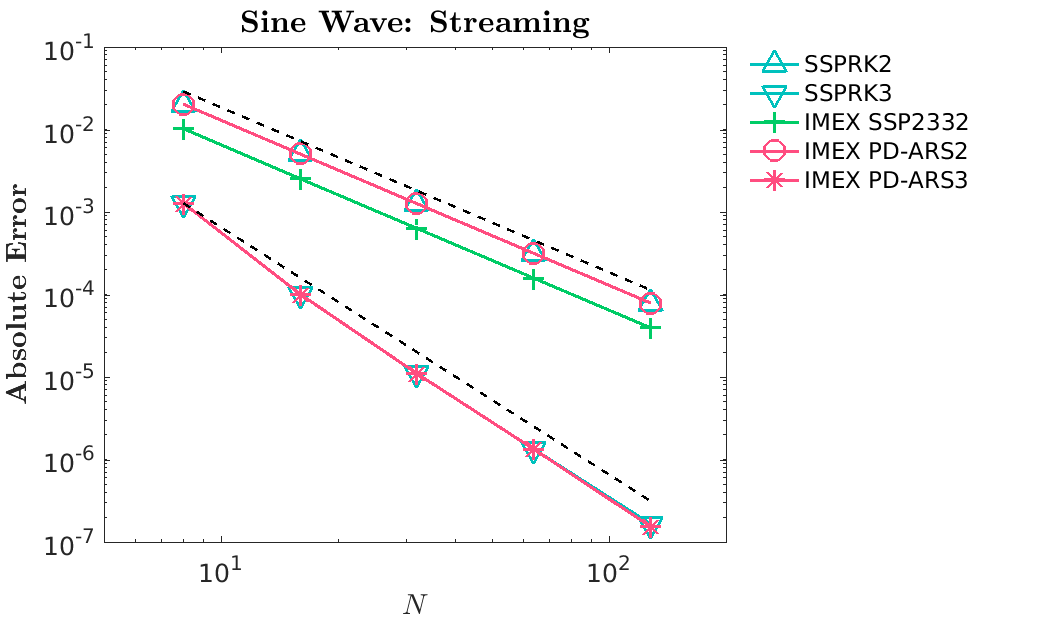
\includegraphics[width=0.6\textwidth]{figures/SineWaveStreaming}
   \caption{Sine Wave Streaming}
\end{figure}

\subsubsection{Sine Wave Damping}
\begin{figure}[h]
  \centering
    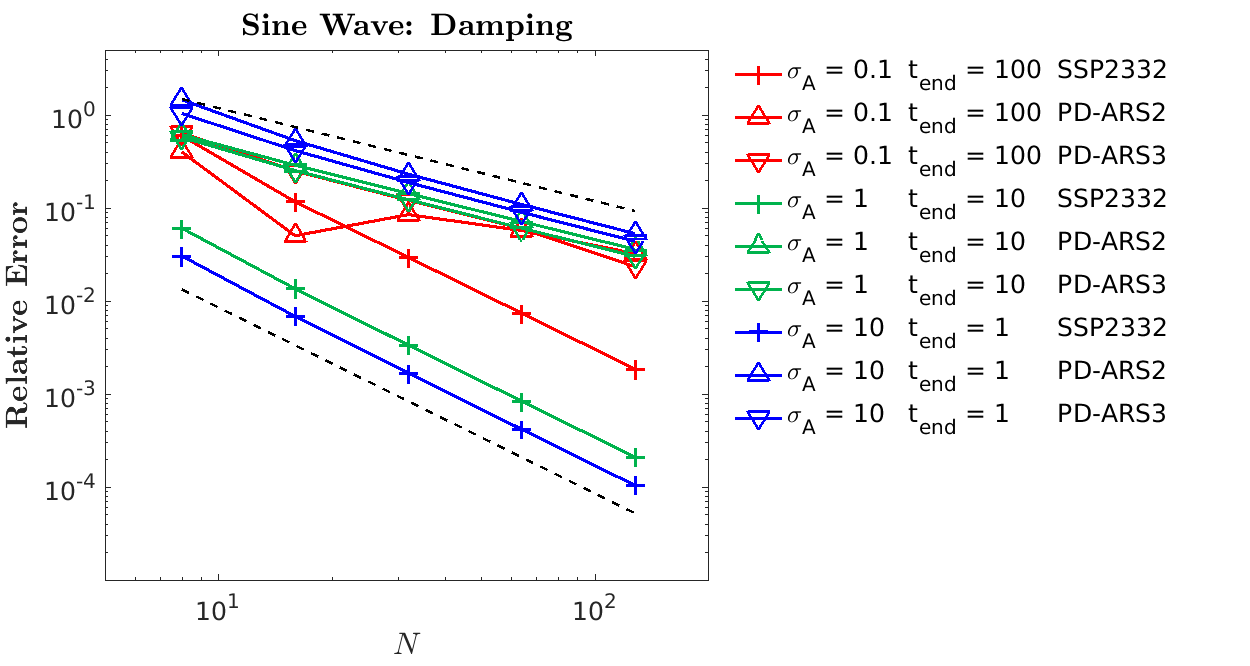
\includegraphics[width=0.7\textwidth]{figures/SineWaveDamping}
   \caption{Sine Wave Damping}
\end{figure}
\subsubsection{Sine Wave Diffusion}
\begin{figure}[h]
  \centering
  \begin{tabular}{cc}
    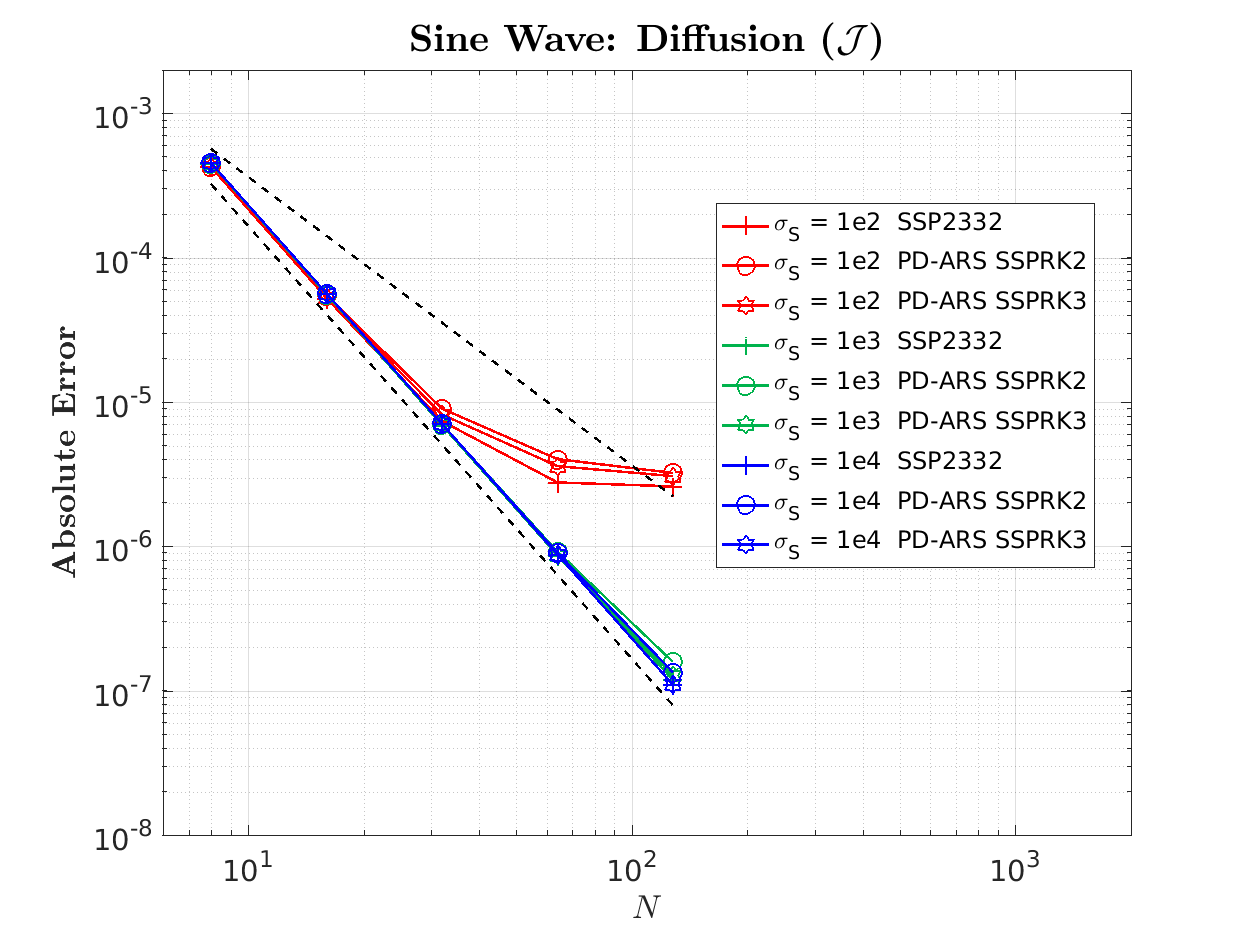
\includegraphics[width=0.5\textwidth]{figures/SineWaveDiffusionJ}
    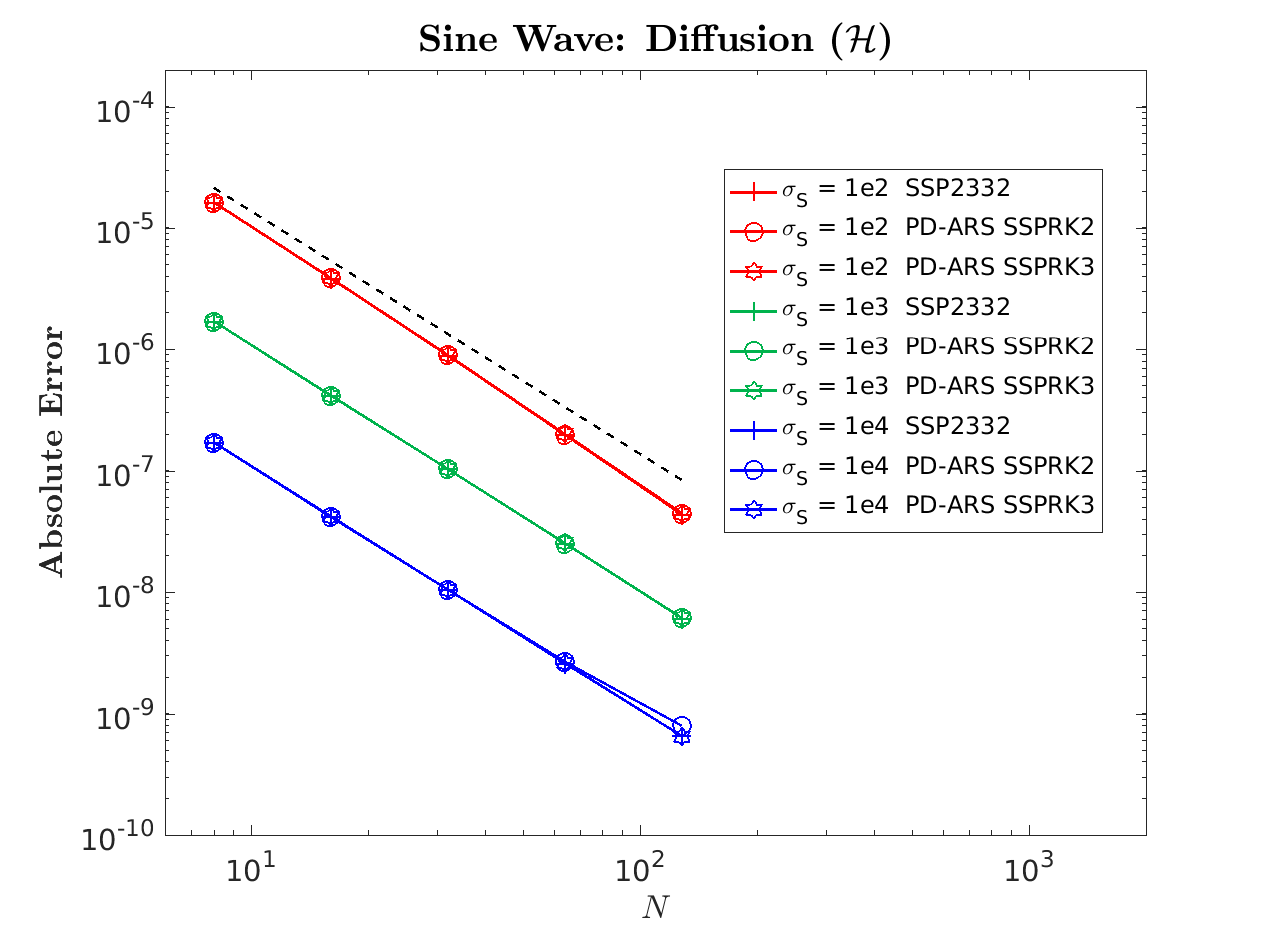
\includegraphics[width=0.5\textwidth]{figures/SineWaveDiffusionH}
  \end{tabular}
   \caption{Sine Wave Diffusion}
\end{figure}

\subsection{Constraint-Preserving Tests}


\subsubsection{Neutrino Stationary State Test}
\begin{figure}[h]
  \centering
  \begin{tabular}{cc}
    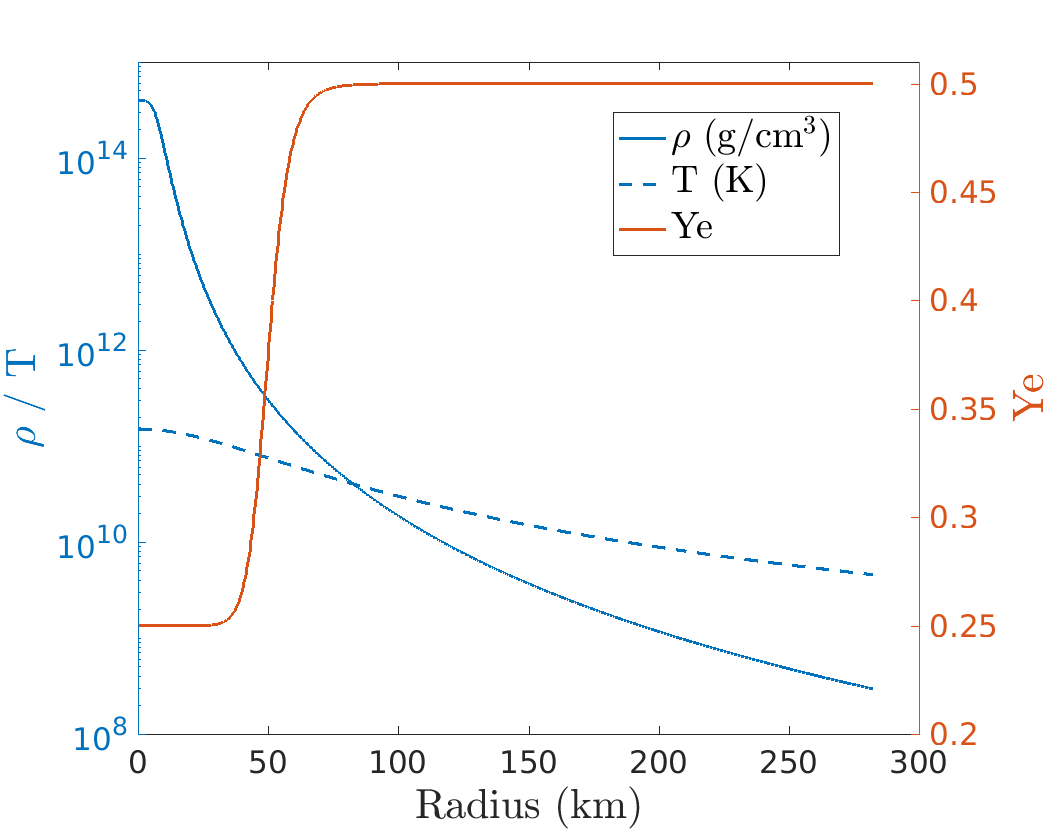
\includegraphics[width=0.4\textwidth]{figures/NStatinaryS_EOS}
    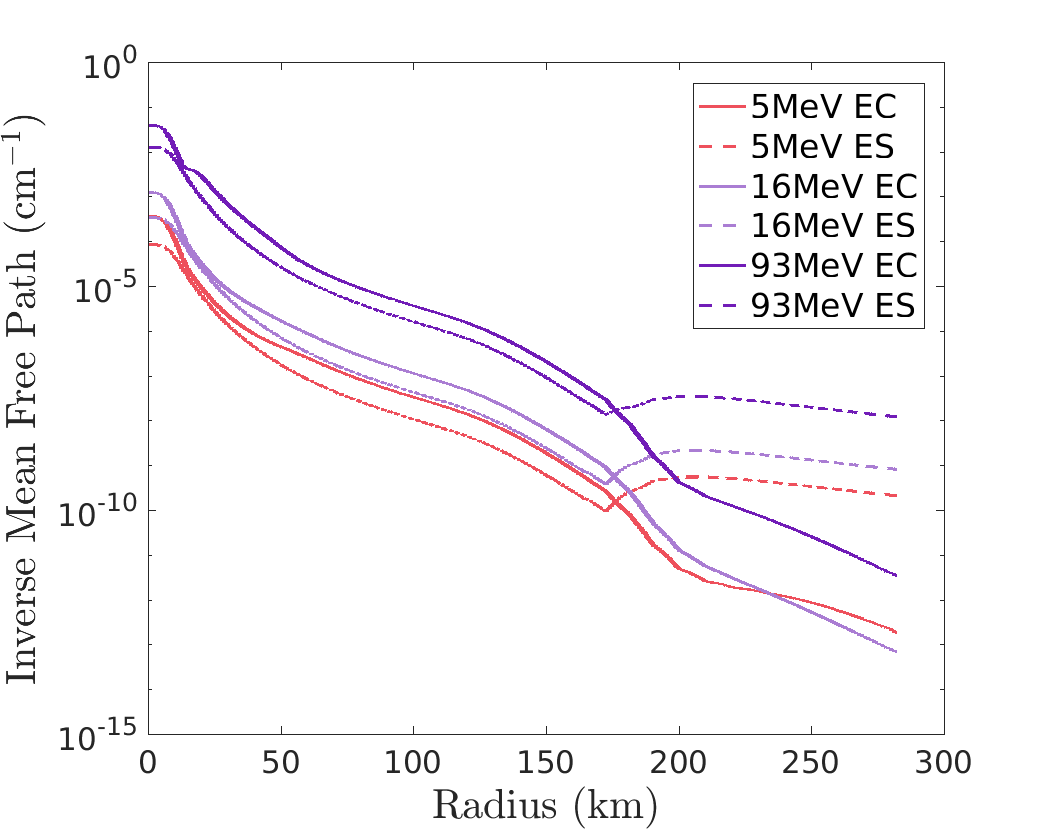
\includegraphics[width=0.55\textwidth]{figures/NSS_Opacities}
  \end{tabular}
   \caption{Neutrino Stationary State Test}
\end{figure}

\begin{figure}[h]
  \centering
  \begin{tabular}{cc}
    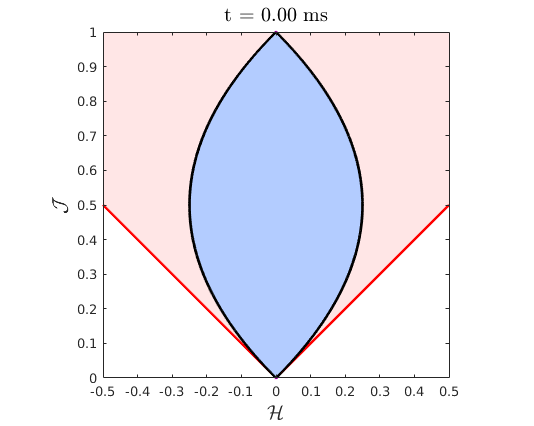
\includegraphics[width=0.45\textwidth]{figures/NSS_0_1}
    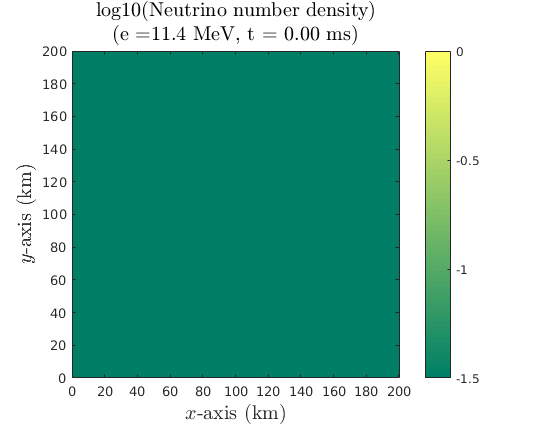
\includegraphics[width=0.45\textwidth]{figures/NSS_0_2} \\
    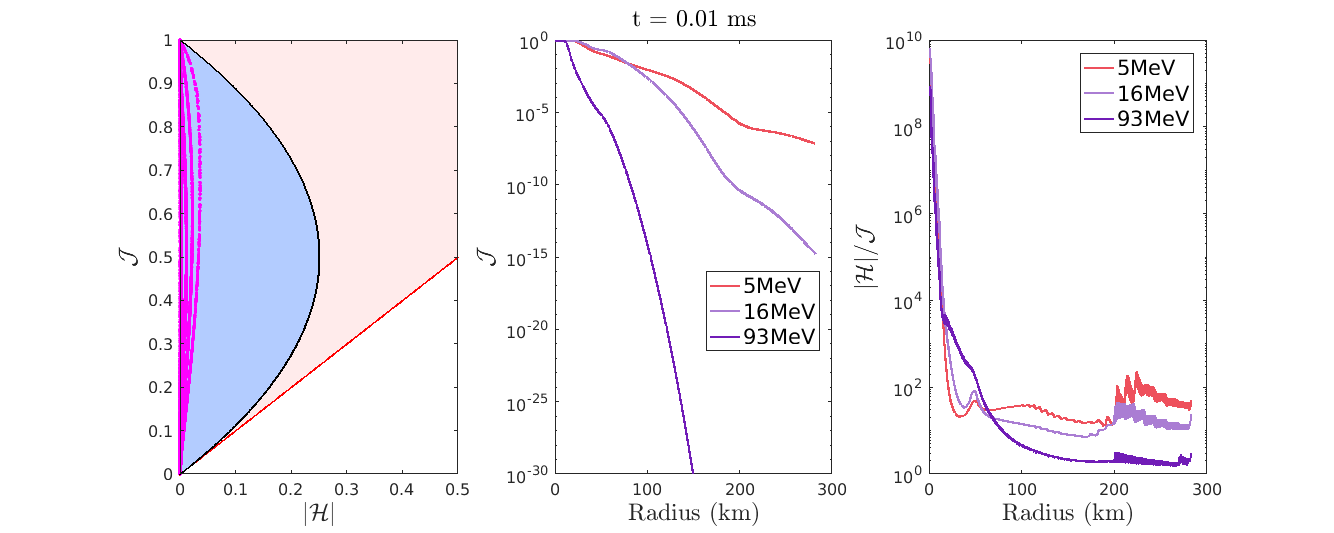
\includegraphics[width=0.45\textwidth]{figures/NSS_1_1}
    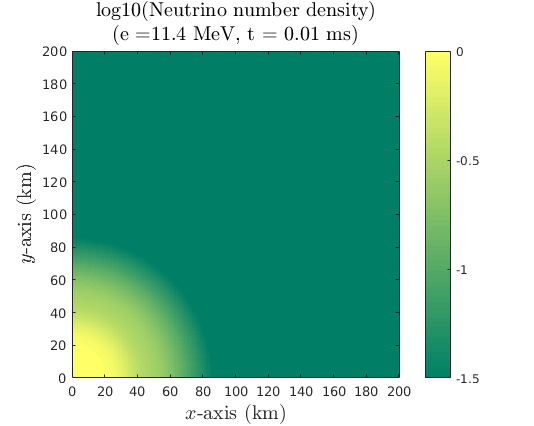
\includegraphics[width=0.45\textwidth]{figures/NSS_1_2} \\
    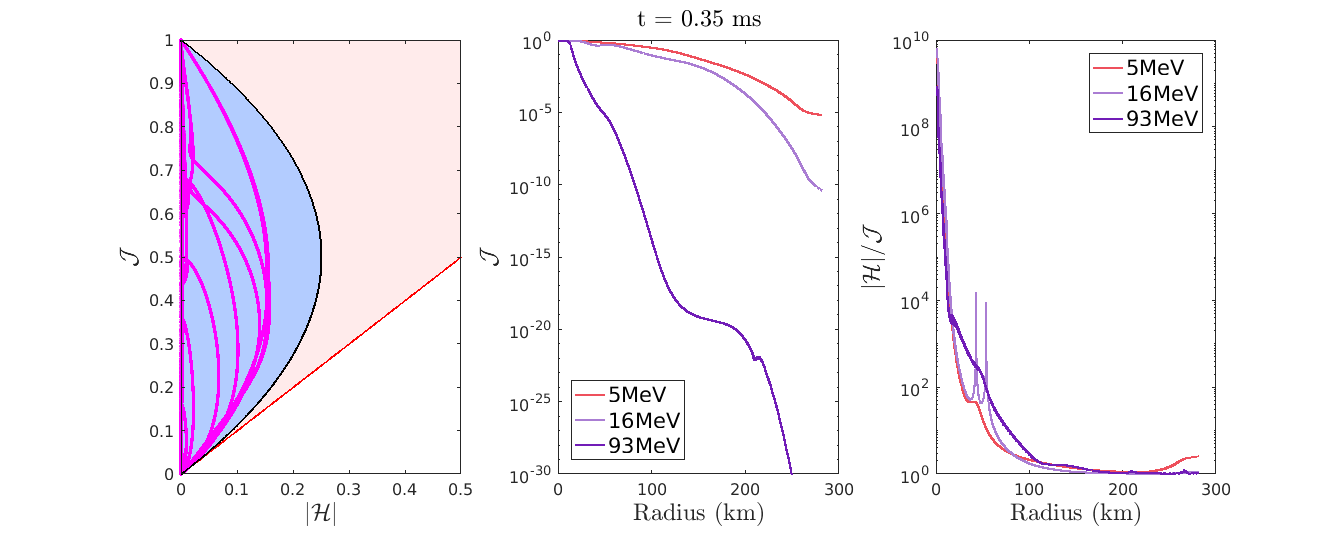
\includegraphics[width=0.45\textwidth]{figures/NSS_3_1}
    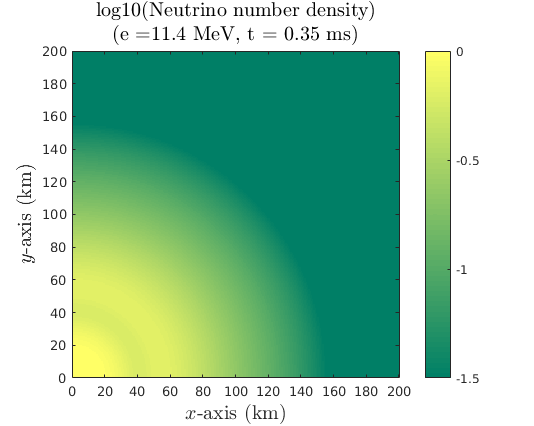
\includegraphics[width=0.45\textwidth]{figures/NSS_3_2} \\
    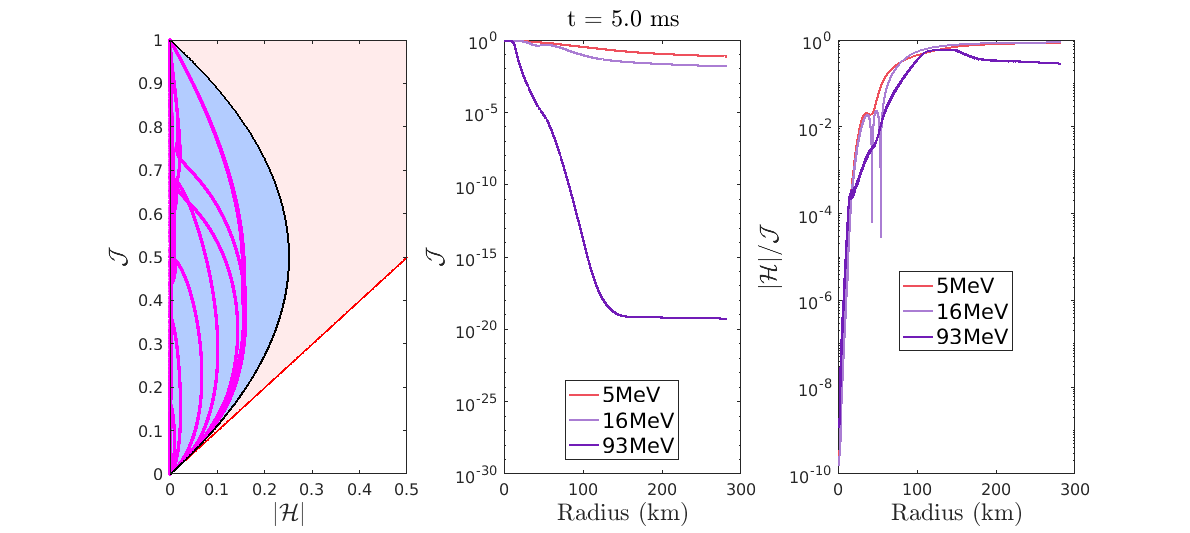
\includegraphics[width=0.45\textwidth]{figures/NSS_5_1}
    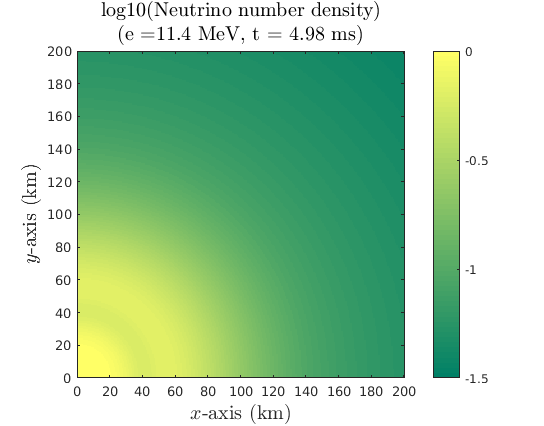
\includegraphics[width=0.45\textwidth]{figures/NSS_5_2} \\
  \end{tabular}
   \caption{Neutrino Stationary State Test}
\end{figure}
\section{Summary and Outlook}\label{se:Summary}

We have developed IMEX schemes suitable for a two-moment model of neutrino transport that obey Fermi-Dirac statistics.
The scheme employs algebraic closure based on Fermi-Dirac statistics, high-order discontinuous Galerkin methods for spatial discretization, and convex-invariant time integration to maintain realizability of the moments.  
Since the realizable domain is convex and its convexity can be inherited by a convex combination, a scheme having convex combinations as its stages can preserve the realizable domain.
This encouraged us to construct realizability-preserving time integrators, realizability-preserving IMEX schemes, and a method with a realizability-preserving IMEX time integrator and high-order DG method.  

In the applications that motivate this work, the neutrino distribution function can vary from 0 to 1.  
Hence, we have considered algebraic closures based on Fermi-Dirac statistics for both low and high occupancy.  
Among the seven algebraic closures we considered -- Kershaw~\cite{kershaw_1976}, Wilson~\cite{wilson_1975,leblancWilson_1970}, Levermore~\cite{levermore_1984}, Minerbo~\cite{minerbo_1978}, Janka 1~\cite{janka_1991}, Janka 2~\cite{janka_1992}, and Cernohorsky \& Bludman~\cite{cernohorskyBludman_1994} -- only the Cernohorsky \& Bludman closure obeys Fermi-Dirac statistics for all occupancies.  
As a result, we employed the Cernohorsky \& Bludman closure for the neutrino stationary state test in Section~\ref{se: Neutrino Stationary State Test}.
We also ran our code with Minerbo closure, IMEX PC2, IMEX SSP2332 and IMEXRKCB2 schemes, and the results show that only PD-ARS schemes have stability.
In addition, closures have impact on the simulation result.
As we observed, both using PD-ARS scheme, there are $\sim30\%$ difference in the neutrino number densities (and relaxation time) between the results obtained with Minerbo closure and that with CB closure.
Even though RKCB2 with Minerbo closure luckily survived our test, the results it gave were compromised: closer to PD-ARS scheme with Minerbo closure other than PD-ARS scheme with CB closure.
In what way and to what degree the results are in fact compromised either by the closure or by a particular correction step for unrealizable moments are difficult to determine fully and is left for further study.


Two PD-ARS schemes are proposed.
The one with SSPRK2 has second-order accuracy while the other with SSPRK3 has third-order accuracy, and both have the strong-stability preserving property in the streaming limit.  
Their accuracy was demonstrated on problems with known smooth solutions in streaming, absorption, and scattering-dominated regimes.
The neutrino transport test with emission, absorption, and isoenergetic scattering through a stationary background, was designed to test the convex-invariance of our PD-ARS schemes. 
The neutrino stationary state test shows that a method combining an algebraic closure based on Fermi-Dirac statistics and convex-invariant time integration is promising for robust CCSN simulation.

In this work, we adopted Cartesian coordinates, a linear collision term, and a fixed material background.
More realistic problems of scientific interest, such as with energy-exchanging scattering and relativistic effects, are left for future research.
\section{Acknowledgment} \label{se:Acknowledgment}

This research is sponsored, in part, by the Laboratory Directed Research and Development Program of Oak Ridge National Laboratory (ORNL), managed by UT-Battelle, LLC for the U. S. Department of Energy under Contract No. De-AC05-00OR22725.  
This research was supported by the Exascale Computing Project (17-SC-20-SC), a collaborative effort of the U.S. Department of Energy Office of Science and the National Nuclear Security Administration.  
This material is based, in part, upon work supported by the U.S. Department of Energy, Office of Science, Office of Advanced Scientific Computing Research.
Eirik Endeve and Anthony Mezzacappa acknowledge support from the National Science Foundation under group NSF-GP-... and from the UT-ORNL Joint Institute for Computational Sciences.

%\section*{References}
\bibliography{references/references}

\end{document}


